% ------------------------------------------------------------------------------------
\newpage
{\color{lightgray} \hrule}
\begin{enumerate} \setcounter{enumi}{2}
	\item Considere el ejemplo referente al número de fallas de bombas de agua en una central nuclear, donde $p_i$ representa el número de fallas en el tiempo de operación $t_i$, con $i= 1,\dots,n$.
	
	Se considera el modelo $p_i \sim Poisson(\lambda_i t_i)$, (las $\lambda_i$ son independientes entre si), con distribuciones a priori $\lambda_i|\beta \sim Gama(\alpha, \beta)$ y $\beta\sim Gama(\gamma,\delta)$, por lo tanto:
	\begin{equation} \label{eq:13}
		f(\lambda_1,\dots,\lambda_n,\beta) = f(\lambda_1|\beta) f(\lambda_2|\beta)\cdots f(\lambda_n|\beta) f(\beta)
	\end{equation}
	Para la distribución posterior se tiene:
	\begin{equation} \label{eq:14}
		f(\lambda_1,\dots,\lambda_n,\beta | \bar{p}) \propto L(\bar{p},\bar{\lambda},\beta) f(\lambda_1,\dots,\lambda_n,\beta)
	\end{equation}
	Simule valores de la distribución posterior $f(\lambda_1,\dots,\lambda_n,\beta | \bar{p})$ usando
	un kernel híbrido, considerando las propuestas:
	\begin{equation} \label{eq:15}
		\lambda_i | \bar{\lambda}_{-i}, \beta, \bar{t} \sim Gama(p_i+\alpha, \beta+t_i)
	\end{equation}
	\begin{equation} \label{eq:16}
		\beta | \bar{\lambda}, \bar{t} \sim Gama\left(n \alpha + \gamma, \delta+ \sum_{i=1}^{n} \lambda_i \right)
	\end{equation}
	Verifique que estas son propuestas Gibbs.
	
	Use los datos del Cuadro 1 con los parámetros a priori $\alpha= 1.8$, $\gamma = 0.01$ y $\delta= 1$.
	
	\begin{table}[h!]
		\centering
		\begin{tabular}{|c|c|c|c|c|c|c|c|c|c|c|}
			\hline
			Bomba ($i$) & 1 & 2 & 3 & 4 & 5 & 6 & 7 & 8 & 9 & 10 \\
			\hline
			T. de uso ($t_i$) & 94.32 & 15.72 & 62.88 & 125.76 & 5.24 & 31.44 & 1.05 & 1.05 & 2.1 & 10.48 \\
			\# de fallas ($p_i$) & 5 & 1 & 5 & 14 & 3 & 20 & 1 & 1 & 4 & 22 \\
			\hline
		\end{tabular}
		\caption{Datos de bombas de agua en centrales nucleares (Robert y Casella,
			p. 385) para el ejemplo 8.3.}
	\end{table}

\end{enumerate}

\textcolor{BrickRed}{\it Respuesta:}

De forma muy similar a los ejercicios anteriores, en el archivo \textcolor{mediumblue}{ejercicio3\_tarea8.py}, se comienza implementando la función \textit{plot\_chains()}, la cual recibe una cadena de Markov simulada y grafica el histograma de cada variable, en este caso, se imprimen todas las $\lambda_i$ juntas y el correspondiente a $\beta$ aparte. Una vez más, gracias a lo general que es la función \textit{METROPOLIS\_HASTINGS\_HYBRID\_KERNELS()} descrita en el ejercicio 1, se vuelve a usar sin hacer ninguna modificación.

A continuación, se define la función \textit{posterior()} la cual implementa la expresión \eqref{eq:14} y las propuestas:
\begin{itemize}
	\item \textit{prop\_lambda\_i\_gen()}  y \textit{prop\_lambda\_i\_pdf()}
	\item \textit{prop\_beta\_gen()} y \textit{prop\_beta\_pdf()}
\end{itemize}
las cuales implementan las propuestas \eqref{eq:15} y \eqref{eq:16} así como su densidad de probabilidad respectiva. Notemos que se tiene una función para $\lambda_i$, al final se hace una lista para contemplar a todos los $i\in\{1,\dots,10\}$

Finalmente, se definen los tiempos de operación $t$ y el número de fallas correspondientes $p$ dados en la tabla y se ejecuta el código principal, en el cual se definen los parámetros dados por el ejercicio, como $\alpha=1.8$, $\gamma=0.01$ y $\delta=1$. El punto $x_0$ inicial se tomó aleatorio en $[0,1]$ por simplicidad y se usaron $15,000$ iteraciones del algoritmo, aunque al generar los histogramas finales, se retiró un burn-in de $2000$ puntos. También, se le dio igual probabilidad de elección a cada una de las propuestas: $\frac{1}{11}$. 

Así, se generaron las listas de funciones generadoras y sus respectivas densidades (terminando con $11$ funciones generadoras, $10$ para $\lambda_i$ y la de $\beta$) para aplicar el algoritmo Metropolis Hastings con Kérneles Híbridos, generando los resultados mostrados a continuación:

\begin{figure}[h!]
	\centering
	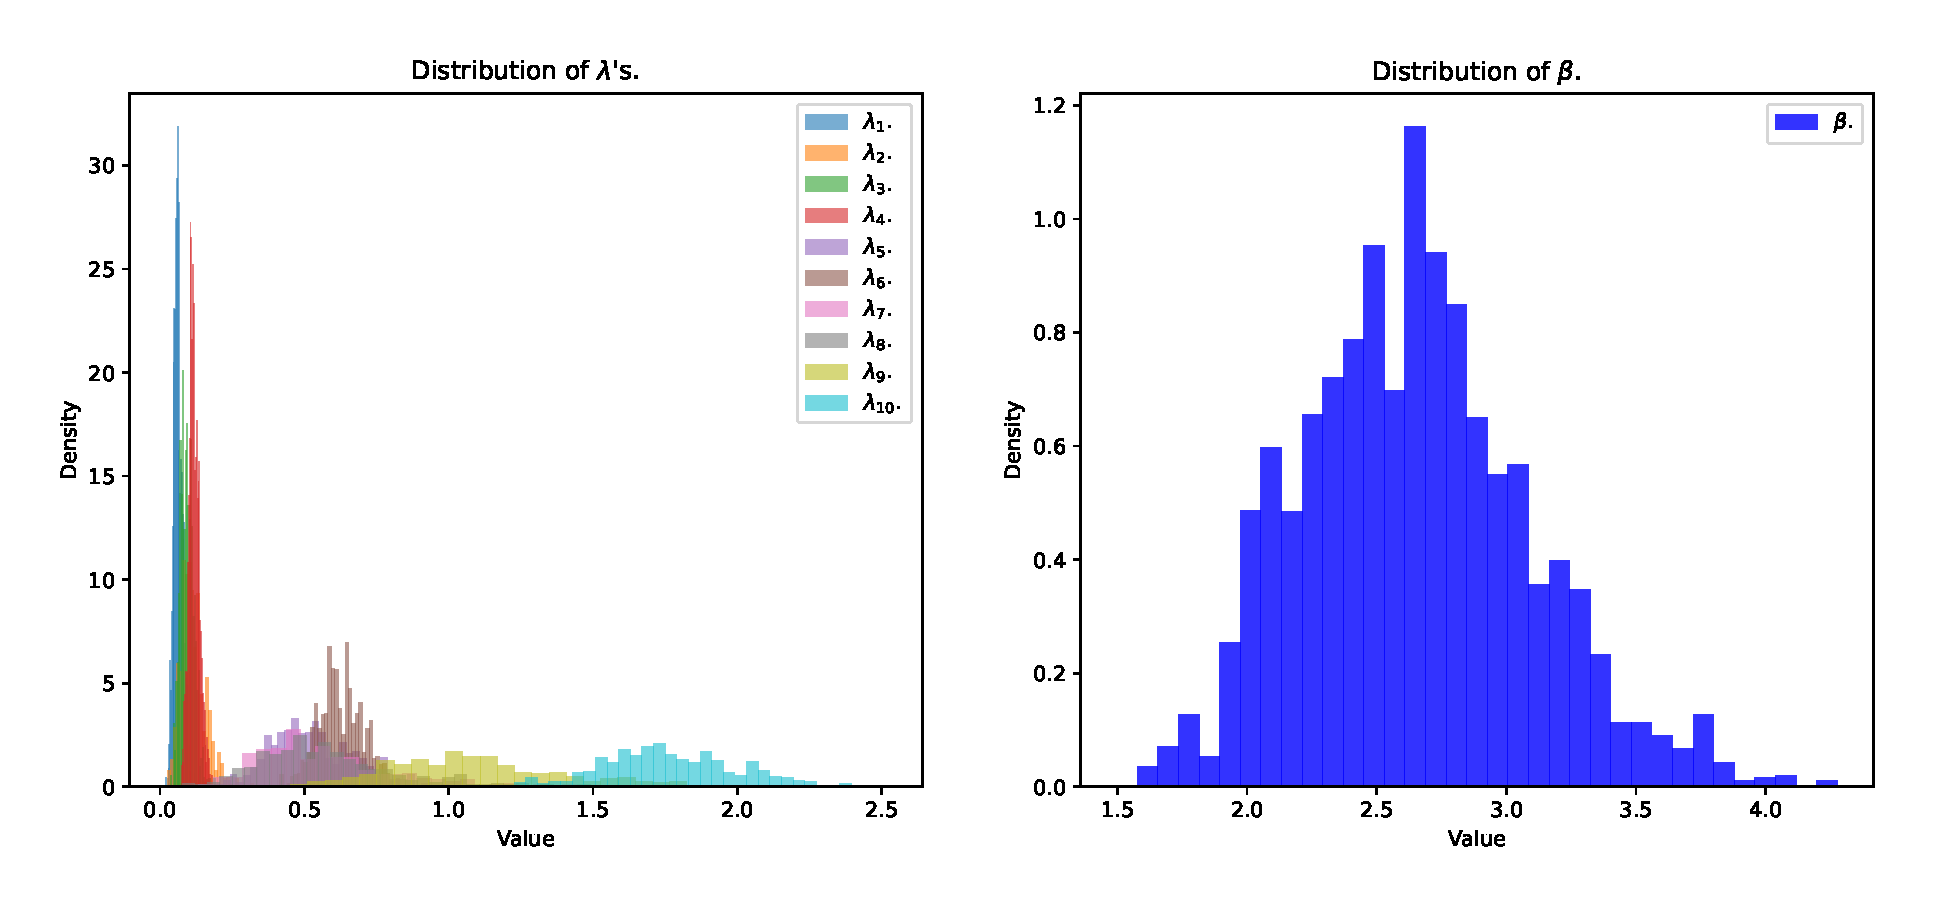
\includegraphics[width=\textwidth]{IMAGENES/exercise3.pdf}
\end{figure}

Tras analizar los resultados generados, la simulación de la distribución posterior  $f(\lambda_1, \dots, \lambda_n, \beta | \bar{p})$  utilizando el kernel híbrido parece haber proporcionado estimaciones razonables para los parámetros $\lambda_i$ y $\beta$.

Las gráficas de densidad para los valores de $\lambda_i$ muestran variabilidad entre las bombas. Esto refleja que las tasas de falla son distintas para cada bomba, posiblemente debido a las diferencias en el tiempo de operación ($t_i$) y el número de fallas observadas ($p_i$). Los valores de $\lambda_i$ para bombas con más fallas y mayor tiempo de operación tienden a ser mayores, lo cual es consistente con el modelo de Poisson.

La distribución posterior de $\beta$ tiene una densidad concentrada, lo que indica que las observaciones proporcionan información suficiente para estimar este parámetro. Esto sugiere que el valor de $\beta$ es estable.

\textbf{Demostración:}

\begin{itemize}
	\item Propuesta para $\lambda_i | \bar{\lambda}_{-i}, \beta, \bar{t}$:
\end{itemize}
Sabemos que $p_i \sim Poisson(\lambda_i t_i)$ y que la distribución a priori de $\lambda_i | \beta$ es $Gama(\alpha, \beta)$. Entonces, la distribución posterior completa de $\lambda_i$ (condicional en $\beta$ y los datos observados) se obtiene como sigue:
\begin{equation}
	f(\lambda_i | p_i, t_i, \beta) \propto f(p_i | \lambda_i, t_i) f(\lambda_i | \beta)
\end{equation}
Sustituyendo las distribuciones, se obtiene:
\begin{equation}
f(\lambda_i | p_i, t_i, \beta) \propto \frac{(\lambda_i t_i)^{p_i} e^{-\lambda_i t_i}}{p_i!} \cdot \frac{\beta^\alpha}{\Gamma(\alpha)} \lambda_i^{\alpha - 1} e^{-\beta \lambda_i}
\end{equation}
Agrupando términos de $\lambda_i$, tenemos:
\begin{equation}
f(\lambda_i | p_i, t_i, \beta) \propto \lambda_i^{p_i + \alpha - 1} e^{-(\beta + t_i) \lambda_i}
\end{equation}
Esta es la forma de una distribución $Gama(p_i + \alpha, \beta + t_i)$, lo cual es precisamente la propuesta indicada en el ejercicio:
\begin{equation}
\lambda_i | \bar{\lambda}_{-i}, \beta, \bar{t} \sim Gama(p_i + \alpha, \beta + t_i)
\end{equation}
Esto demuestra que la propuesta para $\lambda_i$ es la distribución condicional completa, por lo que es una propuesta Gibbs.

\begin{itemize}
	\item Propuesta para $\beta | \bar{\lambda}, \bar{t}$:
\end{itemize}
La distribución a priori de $\beta$ es $Gama(\gamma, \delta)$, y dado que $\lambda_i | \beta \sim Gama(\alpha, \beta)$ para cada $i$, la posterior completa de $\beta$ se obtiene multiplicando estas distribuciones.
La verosimilitud conjunta de $\lambda_i$ dado $\beta$ es:
\begin{equation}
f(\lambda_1, \dots, \lambda_n | \beta) = \prod_{i=1}^n \frac{\beta^\alpha}{\Gamma(\alpha)} \lambda_i^{\alpha - 1} e^{-\beta \lambda_i}
\end{equation}
Multiplicando por el prior $f(\beta) \propto \beta^{\gamma - 1} e^{-\delta \beta}$, la distribución posterior de $\beta$ es:
\begin{equation}
f(\beta | \bar{\lambda}, \bar{t}) \propto \beta^{n \alpha + \gamma - 1} e^{-(\delta + \sum_{i=1}^n \lambda_i) \beta}
\end{equation}
Esto es una $Gama(n \alpha + \gamma, \delta + \sum_{i=1}^n \lambda_i)$, que corresponde exactamente a la propuesta:
\begin{equation}
\beta | \bar{\lambda}, \bar{t} \sim Gama(n \alpha + \gamma, \delta + \sum_{i=1}^n \lambda_i)
\end{equation}
Así, también hemos demostrado que esta propuesta para $\beta$ es su distribución condicional completa, confirmando que es una propuesta Gibbs.
